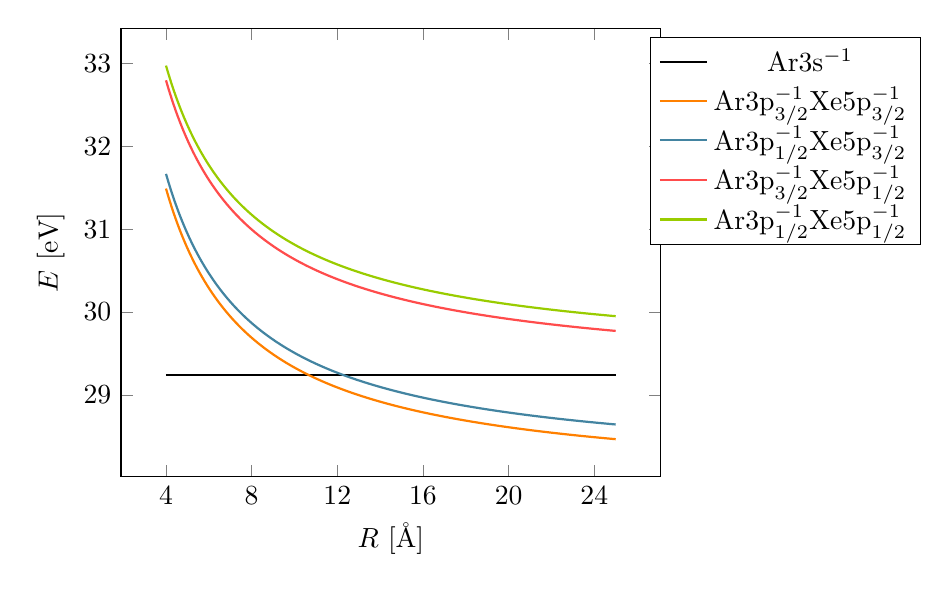
\begin{tikzpicture}
    \begin{axis}[domain=4.0:25,
                 samples = 200,
                 xtick={4.0,8.0,...,24},
                 %xticklabels={$-\pi$,$-\frac \pi 2$,0,$\frac \pi 2$,$\pi$},
                 cycle list name = exotic,
                 legend style={anchor= north west},
                 xlabel={$R$ [\AA]},
                 ylabel={$E$ [eV]}
                 ]
      \addplot+[
                mark = none,
                black,
                thick
               ]
               {29.239};
      \addlegendentry{Ar3s$^{-1}$};
      \addplot+[
                mark = none,
                thick
               ]
               {15.7596 + 12.1298 + 14.39964 / x};
      \addlegendentry{Ar3p$_{3/2}^{-1}$Xe5p$_{3/2}^{-1}$};
      \addplot+[
                mark = none,
                thick
               ]
               {15.9371 + 12.1298 + 14.39964 / x};
      \addlegendentry{Ar3p$_{1/2}^{-1}$Xe5p$_{3/2}^{-1}$};
      \addplot+[
                mark = none,
                thick
               ]
               {15.7596 + 13.4363 + 14.39964 / x};
      \addlegendentry{Ar3p$_{3/2}^{-1}$Xe5p$_{1/2}^{-1}$};
      \addplot+[
                mark = none,
                thick
               ]
               {15.9371 + 13.4363 + 14.39964 / x};
      \addlegendentry{Ar3p$_{1/2}^{-1}$Xe5p$_{1/2}^{-1}$};
      %\draw[] (axis cs:\pgfkeysvalueof{/pgfplots/xmin},29.239) -- (axis cs:\pgfkeysvalueof{/pgfplots/xmax},29.239);
    \end{axis}
\end{tikzpicture}
